\documentclass[]{article}

\usepackage{listings}
\usepackage{float}
\usepackage[margin=1cm]{geometry}
\usepackage{dirtytalk}
\usepackage[x11names, svgnames, rgb]{xcolor}
\usepackage[utf8]{inputenc}
\usepackage{tikz}
\usetikzlibrary{snakes,arrows,shapes}
\usepackage{amsmath}

\definecolor{codegreen}{rgb}{0,0.6,0}
\definecolor{codegray}{rgb}{0.5,0.5,0.5}
\definecolor{codepurple}{rgb}{0.58,0,0.82}
\definecolor{backcolour}{rgb}{0.95,0.95,0.92}

\lstdefinestyle{code}{
    backgroundcolor=\color{backcolour},   
    commentstyle=\color{codegreen},
    keywordstyle=\color{blue},
    numberstyle=\tiny\color{codegray},
    stringstyle=\color{codepurple},
    basicstyle=\ttfamily\footnotesize,
    breakatwhitespace=false,         
    breaklines=true,                 
    captionpos=b,                    
    keepspaces=true,                 
    numbers=left,                    
    numbersep=5pt,                  
    showspaces=false,                
    showstringspaces=false,
    showtabs=false,                  
    tabsize=2
}

\definecolor{delim}{rgb}{0.5,0.5,0}
\definecolor{punct}{rgb}{0,0,0.5}
\definecolor{numb}{rgb}{0,0.5,0.5}

\lstdefinelanguage{json}{
    basicstyle=\normalfont\ttfamily,
    numbers=left,
    numberstyle=\scriptsize,
    stepnumber=1,
    numbersep=8pt,
    showstringspaces=false,
    breaklines=true,
    frame=lines,
    backgroundcolor=\color{backcolour},
    literate=
     *{0}{{{\color{numb}0}}}{1}
      {1}{{{\color{numb}1}}}{1}
      {2}{{{\color{numb}2}}}{1}
      {3}{{{\color{numb}3}}}{1}
      {4}{{{\color{numb}4}}}{1}
      {5}{{{\color{numb}5}}}{1}
      {6}{{{\color{numb}6}}}{1}
      {7}{{{\color{numb}7}}}{1}
      {8}{{{\color{numb}8}}}{1}
      {9}{{{\color{numb}9}}}{1}
      {:}{{{\color{punct}{:}}}}{1}
      {,}{{{\color{punct}{,}}}}{1}
      {\{}{{{\color{delim}{\{}}}}{1}
      {\}}{{{\color{delim}{\}}}}}{1}
      {[}{{{\color{delim}{[}}}}{1}
      {]}{{{\color{delim}{]}}}}{1},
}

\lstset{style=code}

\title{RISC-V approach proposal}
\author{Abdelsalam ElTamawy}


\begin{document}

	% \maketitle

	In essence what we are trying to do is breakup \verb|verilog| code and decidedly put it back together omitting certain parts of it depending on which instructions are used and which \verb|verilog| code is needed to support these instructions.

	First we create classify how each group-able block of \verb|verilog| code is used by each instruction. To communicate that with ourselves and each other, we can simply add comments to each block, or even line if need be, so that we can much more easily identify them.

	\begin{lstlisting}[language=verilog, caption=an example of an annotated file]
		`include "defines.v"

		module alu (
			input [31:0]a // ADD, SUB, SLL, SLT, XOR, OR, SRA, AND, ADDI, SLTI, SLTIU, XORI, ORI, ANDI, SLLI, SRLI, SRLI, SRAI
			, input [31:0]b // // ADD, SUB, SLL, SLT, XOR, OR, SRA, AND, ADDI, SLTI, SLTIU, XORI, ORI, ANDI, SLLI, SRLI, SRLI, SRAI
			, input [4:0]shamt // SLL, SLT, SLTU
			, output reg [31:0]out // all, requirement of the module
			, output cf 
			, input [3:0]alufn // ADD, SUB, SLL, SLT, XOR, OR, SRA, AND, ADDI, SLTI, SLTIU, XORI, ORI, ANDI, SLLI, SRLI, SRLI, SRAI
			);
		
			wire [31:0] add, op_b; // ADD, SUB
			
			assign op_b = (~b); // SUB
			
			assign {cf, add} = alufn[0] ? (a + op_b + 1'b1) : (a + b); // ADD, SUB
			
			assign vf = (a[31] ^ (op_b[31]) ^ add[31] ^ cf);
			
			wire[31:0] sh; // SLLI, SRLI, SRAI, SLL, SLT, SLTU
			shifter shifter0(.a(a), .shamt(shamt), .type(alufn[1:0]),  .r(sh)); // SLLI, SRLI, SRAI, SLL, SLT, SLTU
			
			always @ * begin
				out = 0;
				(* parallel_case *)
				case (alufn)
					// arithmetic
					`ALU_ADD : out = add;
					`ALU_SUB : out = add;
					`ALU_PASS : out = b;
					// logic
					`ALU_OR:  out = a | b;
					`ALU_AND:  out = a & b;
					`ALU_XOR:  out = a ^ b;
					// shift
					`ALU_SRL:  out=sh;
					`ALU_SRA:  out=sh;
					`ALU_SLL:  out=sh;
					// slt & sltu
					`ALU_SLT:  out = {31'b0,(sf != vf)};
					`ALU_SLTU:  out = {31'b0,(~cf)};
				endcase
			end
		endmodule
	\end{lstlisting}

	Now we have an easy way of immediately identifying code to instruction relations.
	With this classification, we can build a JSON file that represent this.

	\pagebreak
	\begin{lstlisting}[language=json,caption=example JSON]
	{
		"module": "ALU"
		"args": [
			{
				"type": "input", "length": 32, "name": "a",
				"instructions": ["ADD", "SUB", "SLL", "SLT", "XOR", "OR", "SRA", "AND", "ADDI", "SLTI", "SLTIU", "XORI", "ORI", "ANDI", "SLLI", "SRLI", "SRLI", "SRAI"]
			},
			{
				"type": "input", "length": 32, "name": "b",
				"instructions": ["ADD", "SUB", "SLL", "SLT", "XOR", "OR", "SRA", "AND", "ADDI", "SLTI", "SLTIU", "XORI", "ORI", "ANDI", "SLLI", "SRLI", "SRLI", "SRAI"]
			},
			{
				"type": "input", "length": 5, "name": "shamt",
				"instructions": ["SLL", "SLT", "SLTU"]
			},
			{
				"type": "output reg", "length": 32, "name": "out",
				"instructions": ["all"]
			},
			{
				"type": "input", "length": 1, "name": "cf",
				"instruction": ["all"]
			},
			{
				"type": "output", "length": 4, "name": "alufn",
				"instructions": ["ADD", "SUB", "SLL", "SLT", "XOR", "OR", "SRA", "AND", "ADDI", "SLTI", "SLTIU", "XORI", "ORI", "ANDI", "SLLI", "SRLI", "SRLI", "SRAI"]
			}
		]
		"declarations": [
			{
				"type": "wire", "length": 32, "name": "add"
				"instructions": ["ADD", "SUB"]
			},
			{
				"type": "wire", "length": 32, "name": "op_b",
				"instructions": ["SUB"]
			}
		]
		"always": [
			"trigger": "*",
			"case": {
				"condition": "alufn"
				"assigns": [
					{
						"code": "`ALU_ADD : out = add;",
						"req": ["ADD"]
					},
					{
						"code": "`ALU_SUB : out = add;",
						"req": ["SUB"]
					}
					...etc
				]
			}
		]
	}
	\end{lstlisting}

	Using this structure as well as a disjoint set, we can identify only the lines we need and properly output them.

	Here comes the hard part. How to \say{jump through hoops} to completely remove certain components. To do that we can first create a graph to represent where each \say{logical path} leads.
	Then according to that, we can just assign wires to where they are meant to be without modules in the middle.

	\begin{figure}[H]
		\centering
		

	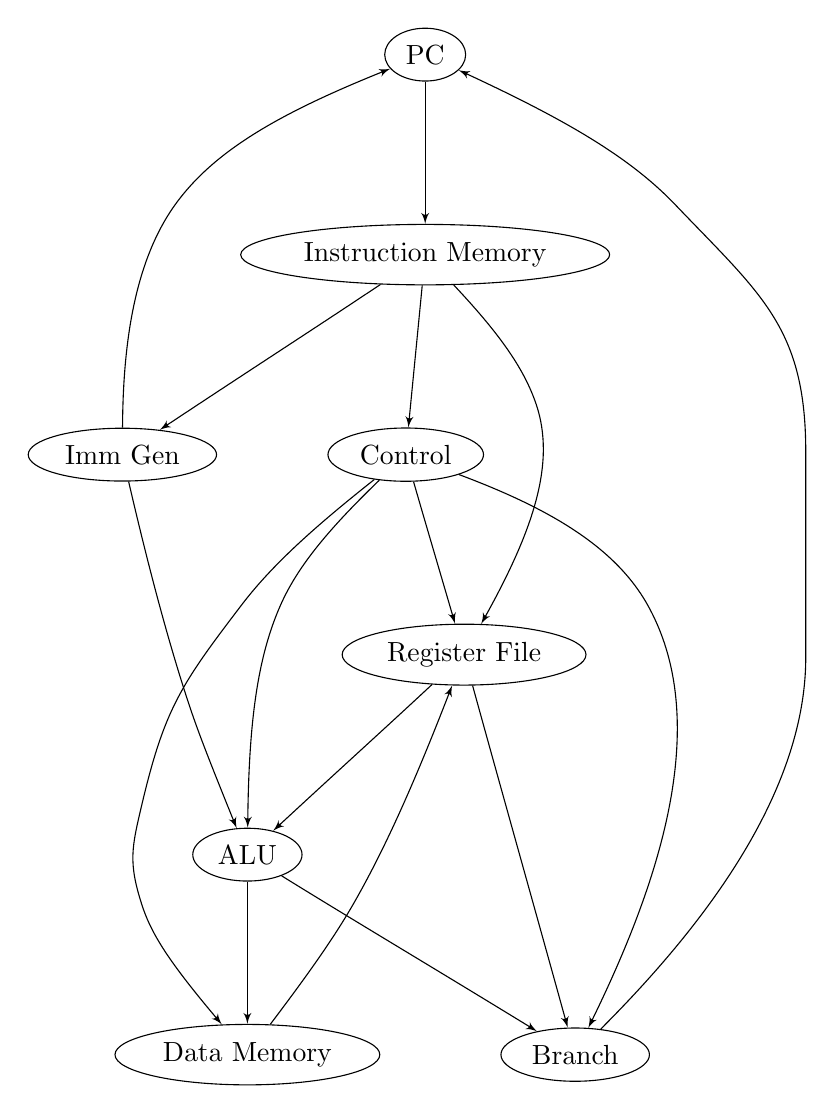
\begin{tikzpicture}[>=latex',line join=bevel]
		\node (pc) at (154.5bp,378.0bp) [draw,ellipse] {PC};
		  \node (im) at (154.5bp,306.0bp) [draw,ellipse] {Instruction Memory};
		  \node (reg) at (168.5bp,162.0bp) [draw,ellipse] {Register File};
		  \node (alu) at (90.496bp,90.0bp) [draw,ellipse] {ALU};
		  \node (br) at (208.5bp,18.0bp) [draw,ellipse] {Branch};
		  \node (dm) at (90.496bp,18.0bp) [draw,ellipse] {Data Memory};
		  \node (imm) at (45.496bp,234.0bp) [draw,ellipse] {Imm Gen};
		  \node (ctrl) at (147.5bp,234.0bp) [draw,ellipse] {Control};
		  \draw [->] (pc) ..controls (154.5bp,351.98bp) and (154.5bp,342.71bp)  .. (im);
		  \draw [->] (reg) ..controls (139.58bp,135.05bp) and (125.71bp,122.6bp)  .. (alu);
		  \draw [->] (reg) ..controls (180.17bp,119.56bp) and (192.77bp,74.819bp)  .. (br);
		  \draw [->] (alu) ..controls (90.496bp,63.983bp) and (90.496bp,54.712bp)  .. (dm);
		  \draw [->] (alu) ..controls (128.81bp,66.272bp) and (156.16bp,50.048bp)  .. (br);
		  \draw [->] (dm) ..controls (111.47bp,45.775bp) and (121.15bp,59.243bp)  .. (128.5bp,72.0bp) .. controls (140.19bp,92.317bp) and (150.93bp,116.67bp)  .. (reg);
		  \draw [->] (br) ..controls (249.08bp,58.636bp) and (291.5bp,108.74bp)  .. (291.5bp,161.0bp) .. controls (291.5bp,235.0bp) and (291.5bp,235.0bp)  .. (291.5bp,235.0bp) .. controls (291.5bp,279.73bp) and (275.39bp,291.65bp)  .. (244.5bp,324.0bp) .. controls (228.18bp,341.09bp) and (205.16bp,354.51bp)  .. (pc);
		  \draw [->] (imm) ..controls (45.684bp,271.24bp) and (49.07bp,302.59bp)  .. (64.496bp,324.0bp) .. controls (78.463bp,343.38bp) and (101.89bp,356.85bp)  .. (pc);
		  \draw [->] (imm) ..controls (53.89bp,197.71bp) and (61.333bp,168.61bp)  .. (69.496bp,144.0bp) .. controls (72.453bp,135.09bp) and (76.102bp,125.5bp)  .. (alu);
		  \draw [->] (ctrl) ..controls (154.92bp,208.26bp) and (157.75bp,198.82bp)  .. (reg);
		  \draw [->] (ctrl) ..controls (120.38bp,207.78bp) and (108.88bp,194.33bp)  .. (102.5bp,180.0bp) .. controls (93.841bp,160.57bp) and (91.003bp,136.56bp)  .. (alu);
		  \draw [->] (ctrl) ..controls (115.32bp,208.51bp) and (99.681bp,194.67bp)  .. (88.496bp,180.0bp) .. controls (66.808bp,151.55bp) and (60.716bp,142.82bp)  .. (52.496bp,108.0bp) .. controls (48.82bp,92.428bp) and (47.6bp,87.232bp)  .. (52.496bp,72.0bp) .. controls (55.77bp,61.814bp) and (61.805bp,51.926bp)  .. (dm);
		  \draw [->] (ctrl) ..controls (198.19bp,215.02bp) and (222.54bp,201.28bp)  .. (234.5bp,180.0bp) .. controls (258.6bp,137.09bp) and (237.98bp,78.214bp)  .. (br);
		  \draw [->] (im) ..controls (180.43bp,278.41bp) and (189.96bp,265.55bp)  .. (194.5bp,252.0bp) .. controls (201.53bp,231.01bp) and (193.5bp,206.88bp)  .. (reg);
		  \draw [->] (im) ..controls (113.72bp,278.81bp) and (93.753bp,265.99bp)  .. (imm);
		  \draw [->] (im) ..controls (151.99bp,279.98bp) and (151.07bp,270.71bp)  .. (ctrl);
		
	\end{tikzpicture}
		\caption{}
		\label{}
	\end{figure}

	A possible way to think about this is to make a sort of optimization passes. For instance, first we remove unnecessary modules.
	then we remove unused multiplexer.

	A good example of this would be how we might not need the data memory module. Then we can realize through the JSON files that we do not need any of the module's internals internals.
	Then using the graph of the datapath, we can determine which wires need to jump to where so that we retain remaining functionality.

\end{document}